\documentclass[12pt,a4paper]{article}

\usepackage[utf8]{inputenc}
\usepackage[brazilian]{babel}
\usepackage{amsmath}
\usepackage{graphicx}
\usepackage{longtable}
\usepackage{siunitx}
\usepackage{booktabs}
\usepackage{geometry}
\usepackage{float}
\usepackage{indentfirst}
\usepackage{newtxtext}
\usepackage{newtxmath}

\usepackage[authoryear]{natbib}

\geometry{margin=2.5cm}

\title{Análise do Movimento Harmônico Amortecido}
\author{Enzo Rocha Leite Diniz Ribas \\ Centro Federal de Educação Tecnológica de Minas Gerais}
\date{\today}

\begin{document}
\begin{titlepage}

\begin{center}


\includegraphics[width=4cm]{media/Logo_CEFET-MG.png}

\Large
Centro Federal de Educação Tecnológica de Minas Gerais

\vspace{1cm}

\Large
Curso de Engenharia Mecânica

\vspace{2cm}

\Huge
Determinação da aceleração da gravidade a partir do movimento oscilatório de um pêndulo simples.

\vspace{3cm}

\begin{flushright}
\Large
Mecânica, Oscilações, Fluidos e Termodinâmica, Turma T03 \\
Prof. Dr. Mauro Lucio Lobão Iannini
\end{flushright}

\vspace{3cm}

\large
Enzo Rocha Leite Diniz Ribas (Eng. Mecânica - 20253002819)\\
Gabriel Resende Amorim Oliveira (Eng. Elétrica - 20233014438)\\
Leandro Césari e Silva Barros (Eng. Mecânica - 20253005104)\\

\vfill

\Large
Belo Horizonte

\Large
\the\year/{1}

\end{center}

\end{titlepage}

\section{Introdução}

O roteiro do experimento \citep{Roteiro_Experimento_05} propõe a análise do movimento harmônico amortecido com o objetivo de ``Analisar a dependência com o tempo da amplitude do movimento harmônico de um sistema massa-mola amortecido'' e ``determinar o coeficiente de amortecimento e outras constantes descritivas do movimento oscilatório''.

\section{Fundamentação Teórica}

\begin{figure}[H]
\centering
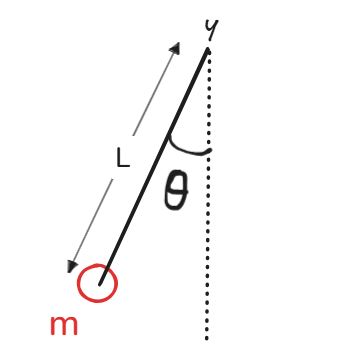
\includegraphics[width=0.8\textwidth]{media/graphs/diagrama}
\caption{Diagrama de um sistema de pêndulo simples. Fonte: Autor}
\label{fig:free_body_diagram}
\end{figure}

\section{Metodologia}

O experimento foi realizado utilizando um sistema de pêndulo simples, composto por uma massa $m$ pendente de um fio de comprimento $L$. O sistema foi configurado para a contagem do período de oscilação do pêndulo para pequenos ângulos de oscilação.

\begin{figure}[H]
\centering
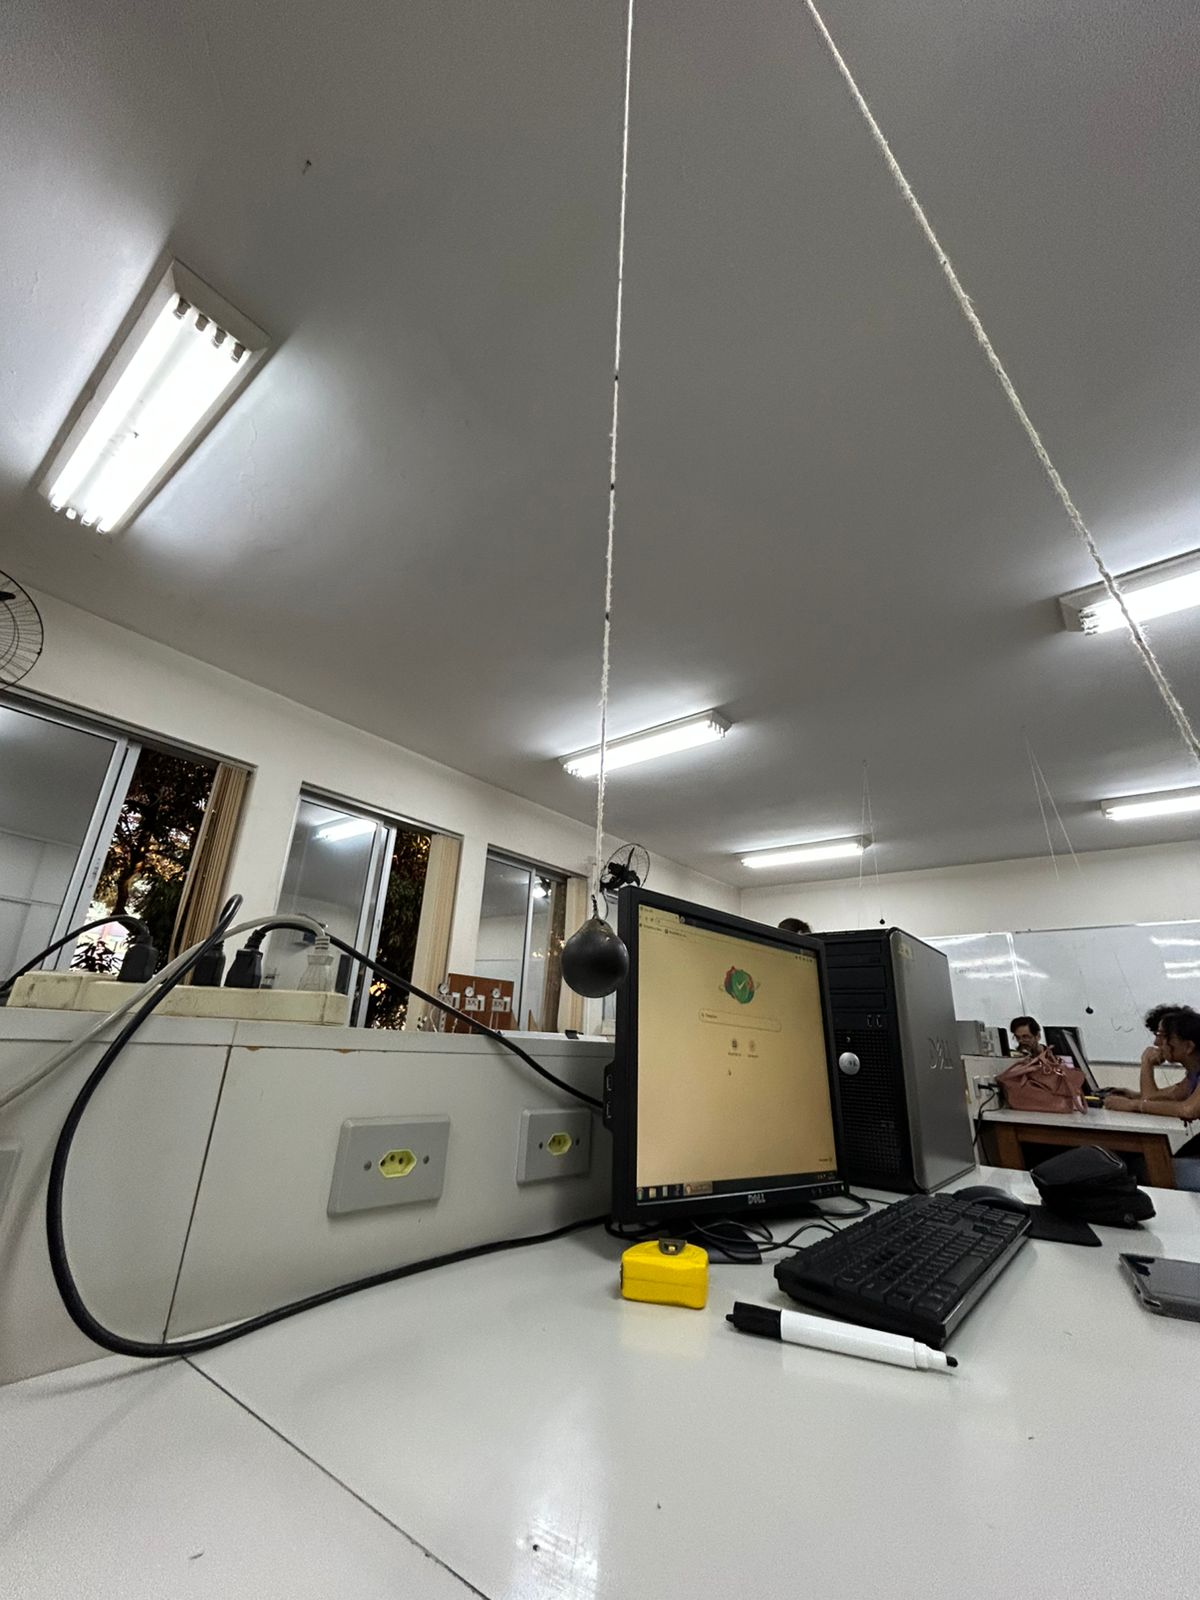
\includegraphics[width=0.8\textwidth]{media/photos/pendulo.png}
\caption{Sistema de pêndulo simples. Fonte: Autor}
\label{fig:pendulo_experimento}
\end{figure}

\begin{figure}[H]
\centering
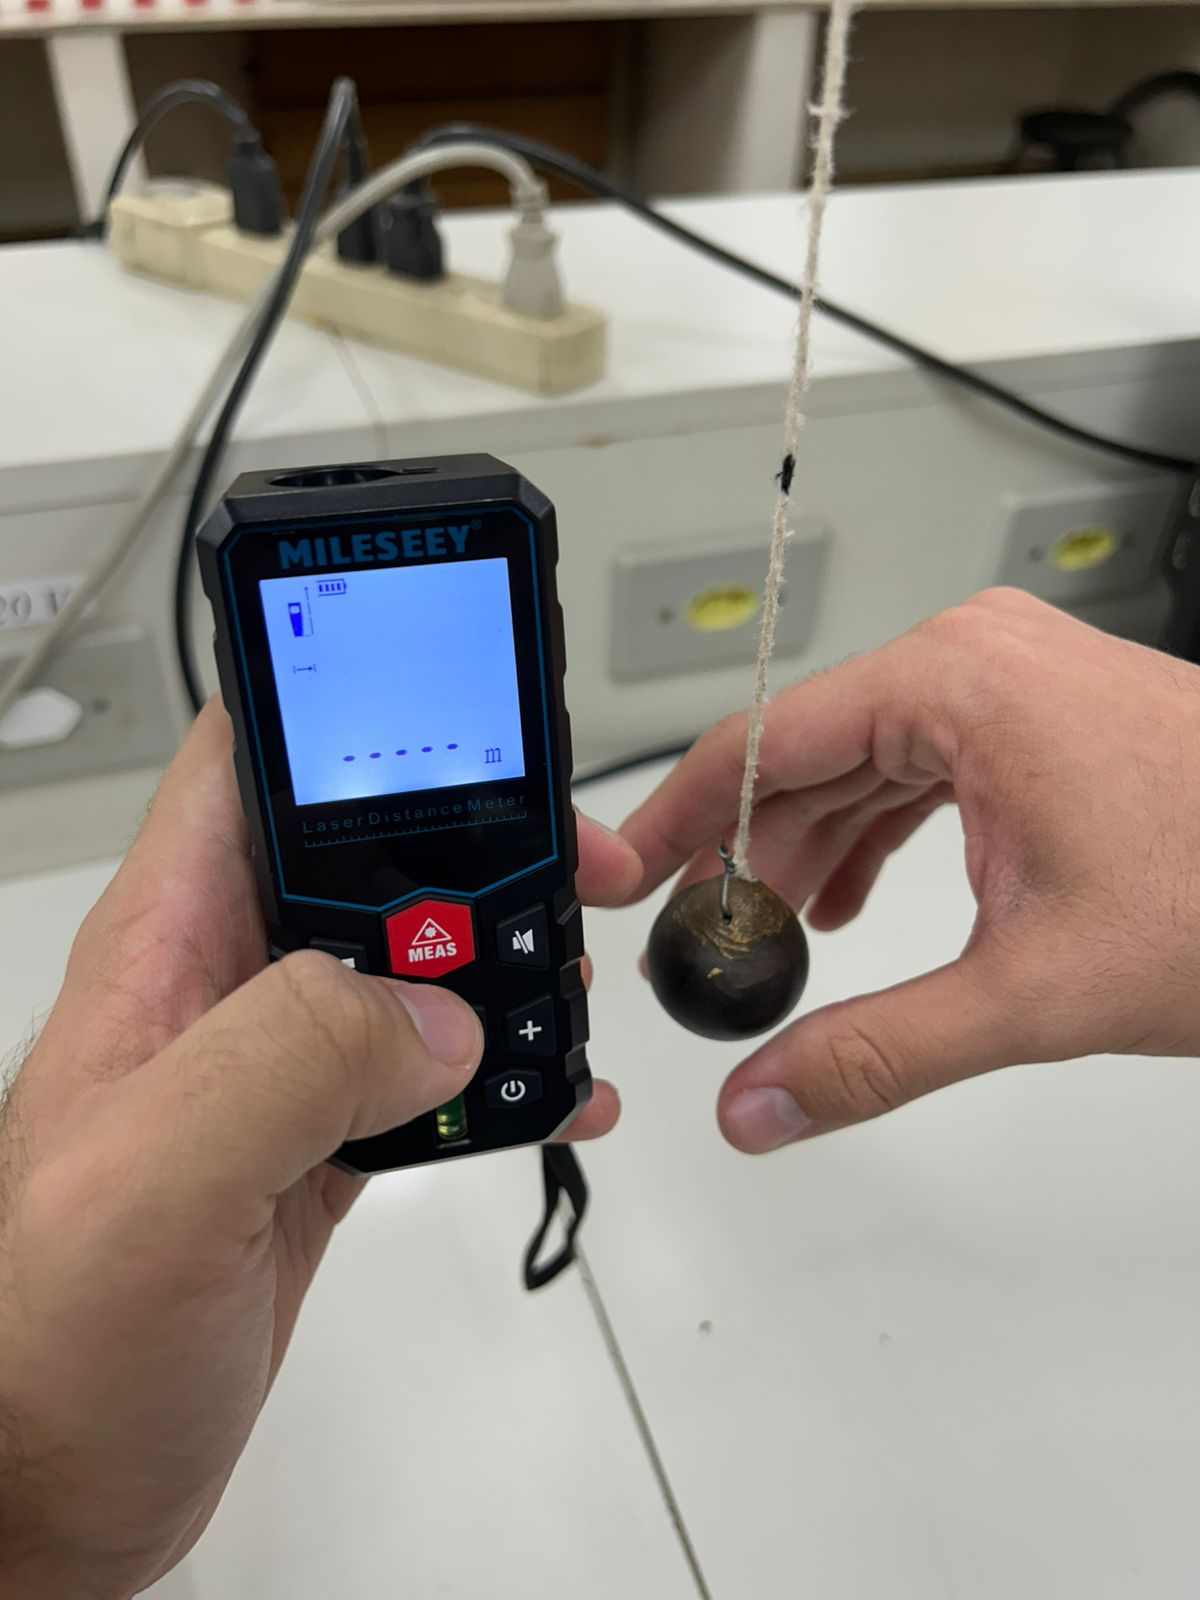
\includegraphics[width=0.8\textwidth]{media/photos/trena_digital.png}
\caption{Trena digital. Fonte: Autor}
\label{fig:trena_digital}
\end{figure}

Os dados do experimento foram anotados em uma tabela para cada comprimento do fio, e posteriormente, a partir dos dados coletados, foi possível determinar a aceleração da gravidade $g$ utilizando o software SciDAVis para análise dos dados e construção de gráficos a partir da linearização dos dados coletados.

\section{Procedimentos}

O procedimento experimental seguiu as seguintes etapas:

\subsection{Construção do experimento}

O sistema foi configurado de maneira que o sistema massa-mola esteja bem fixado e o sensor esteja posicionado de modo a garantir a leitura de todo o movimento, sem obstruções ou interferências.

A frequência utilizada para a aquisição de dados foi de \(100\,\text{Hz}\), o que é suficiente para capturar o movimento oscilatório do sistema massa-mola com precisão.

\subsection{Aquisição do movimento}

O movimento oscilatório foi iniciado e a aquisição de dados foi realizada pelo equipamento e registrada no software \textit{DataStudio}.

\subsection{Filtragem dos dados}

Após a construção da curva no \textit{DataStudio}, foi necessário avaliar se o gráfico obtido está de acordo com o comportamento esperado. Nos casos em que a curva não apresentou o comportamento esperado, foi necessário ajustar o experimento e repetir a aquisição de dados para obter uma curva que se encaixe no modelo teórico do movimento harmônico amortecido.

Além disso, é preciso filtrar os dados exportados do software para garantir que eles se iniciem em um ponto de máxima amplitude, pois isso será crucial para a obtenção dos coeficientes de amortecimento. Caso a curva comece antes ou depois desse ponto, será necessário remover esses dados e reajustar a variável tempo, de modo a obter a curva conforme orientado.

\subsubsection{Construção de gráficos e realização de ajustes no SciDAVis}

No software \textit{SciDAVis}, os dados foram inseridos em uma tabela e utilizados para a construção de um gráfico do tipo \textit{scatter plot}. Com um ajuste (\textit{fit}) com a seguinte fórmula:

\begin{equation}
    \text{* Fórmula usada aqui *}
\end{equation}

Como resultado, obtém-se a curva ajustada aos pontos experimentais e os coeficientes fornecidos no \textit{log} do \textit{SciDAVis}.

 ATUALIZAR AQUI COM A FÓRMULA USADA PARA O AJUSTE LINEAR, QUE DEPENDE DO MODELO ESCOLHIDO (COM OU SEM CONSTANTE DE AJUSTE).
Foram plotados dois gráficos, um considerando a constante de ajuste $b$ como um parâmetro a ser determinado, e outro considerando a constante de ajuste $b$ igual a zero, para comparar os resultados obtidos com os dois modelos de ajuste linear.

A partir dos coeficientes dos ajustes lineares calculados experimentalmente, 
foi possível determinar o módulo da aceleração da gravidade $g$.

\section{Apresentação dos Resultados}

\subsection{Dados Coletados}
Os dados coletados no experimento do pêndulo estão organizados na Tabela~\ref{tab:dados}, que apresenta os valores do comprimento do fio $L$ e o período de oscilação $T$ para cada configuração do experimento.

\begin{table}[H]
\centering
\begin{tabular}{S[table-format=1.3] S[table-format=1.3]}
\toprule
\multicolumn{1}{c}{\shortstack{\textbf{Comprimento do fio} \\ \textbf{$L$ (m)}}} & \multicolumn{1}{c}{\shortstack{\textbf{Período de oscilação} \\ \textbf{$T$ (s)}}} \\
\midrule
2,714 & 1,9 \\
2,507 & 1,648 \\
2,338 & 1,338 \\
2,21 & 1,177 \\
2,046 & 1,036 \\
1,912 & 0,877 \\
1,603 & 0,613 \\
\bottomrule
\end{tabular}
\caption{Dados coletados no experimento do pêndulo.}
\label{tab:dados}
\end{table}

\subsection{Análise dos Dados}

\subsubsection{Ajuste Linear com constante de ajuste}
\begin{figure}[H]
\centering
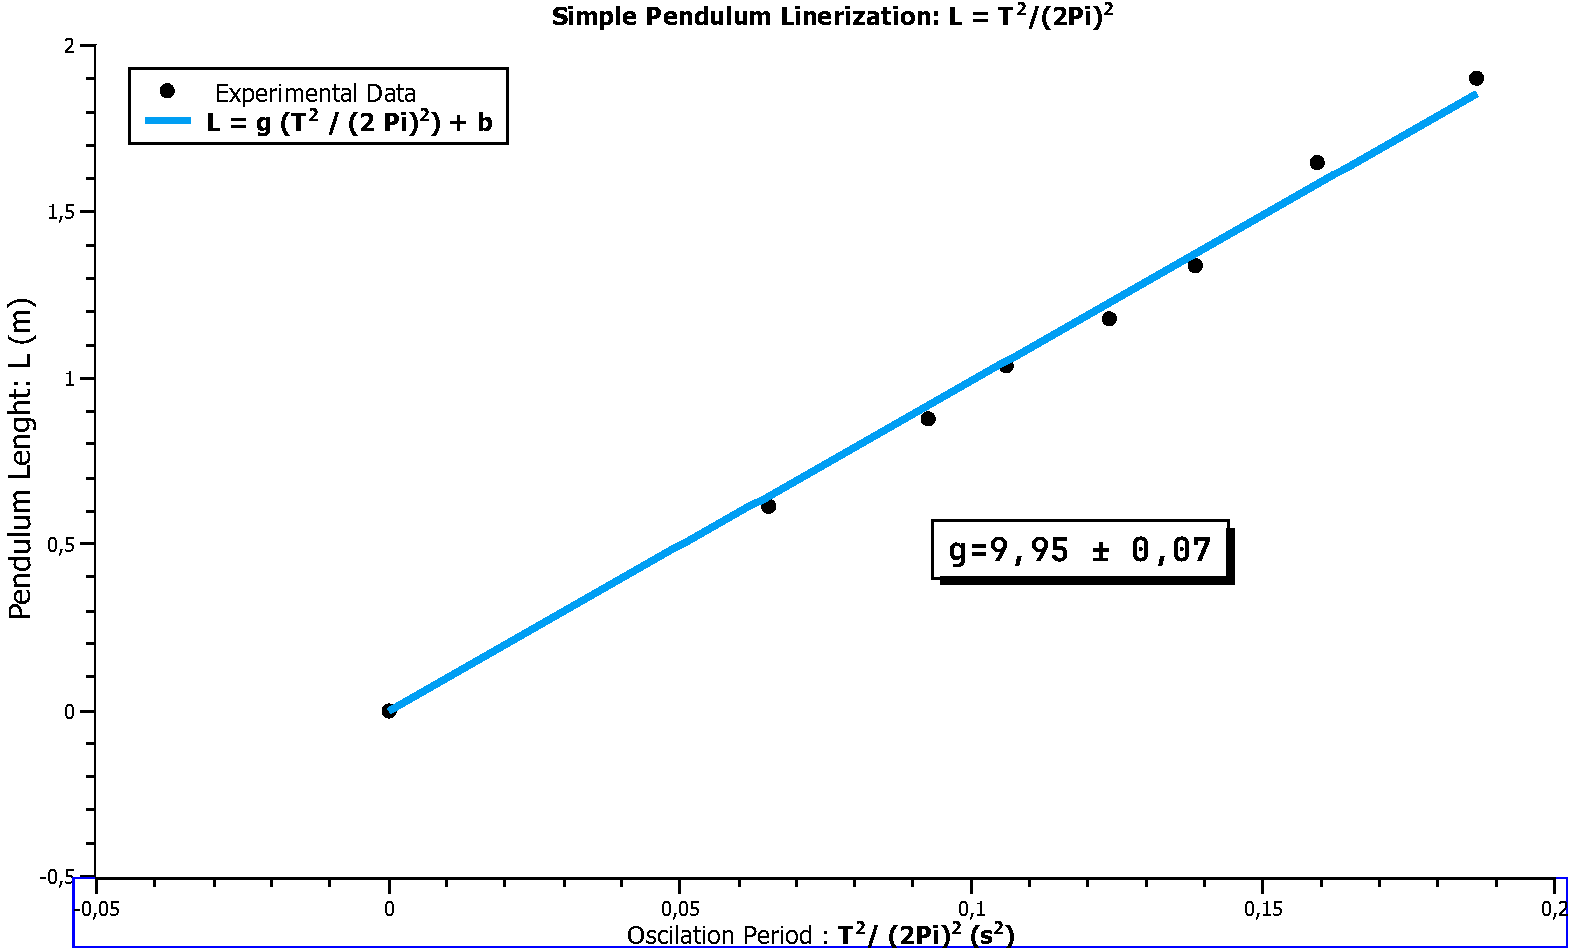
\includegraphics[width=0.8\textwidth]{media/graphs/pendulum_l_2.pdf}
\caption{Ajuste Linear com constante de ajuste. Fonte: Autor}
\label{fig:ajuste_linear_com_constante}
\end{figure}

\subsubsection{Log do SciDAVis}

\begin{verbatim}
[sábado, 25 de abril de 2026 11:25:28 Hora oficial do Brasil	Plot: ''Graph2'']
Non-linear fit of dataset: Table1_l, using function: a*x+b
Y standard errors: Unknown
Scaled Levenberg-Marquardt algorithm with tolerance = 0,0001
From x = 0 to x = 0,186577792296999
a  = 9,95209039767433 +/- 0,0725741275922127
b  = -0,00286887082110515 +/- 0,00456484662317083
--------------------------------------------------------------------------------------
Chi^2 = 0,0137685420208305
R^2 = 0,998825176745932
---------------------------------------------------------------------------------------
Iterations = 1
Status = success
---------------------------------------------------------------------------------------
\end{verbatim}

Valor encontrado de g a partir do ajuste linear com a constante de ajuste: $g = 9,95 \pm 0,07 \, m/s^2$ e constante de ajuste $b = -0,002 \pm 0,004$.

\subsubsection{Ajuste Linear sem constante de ajuste}
\begin{figure}[H]
\centering
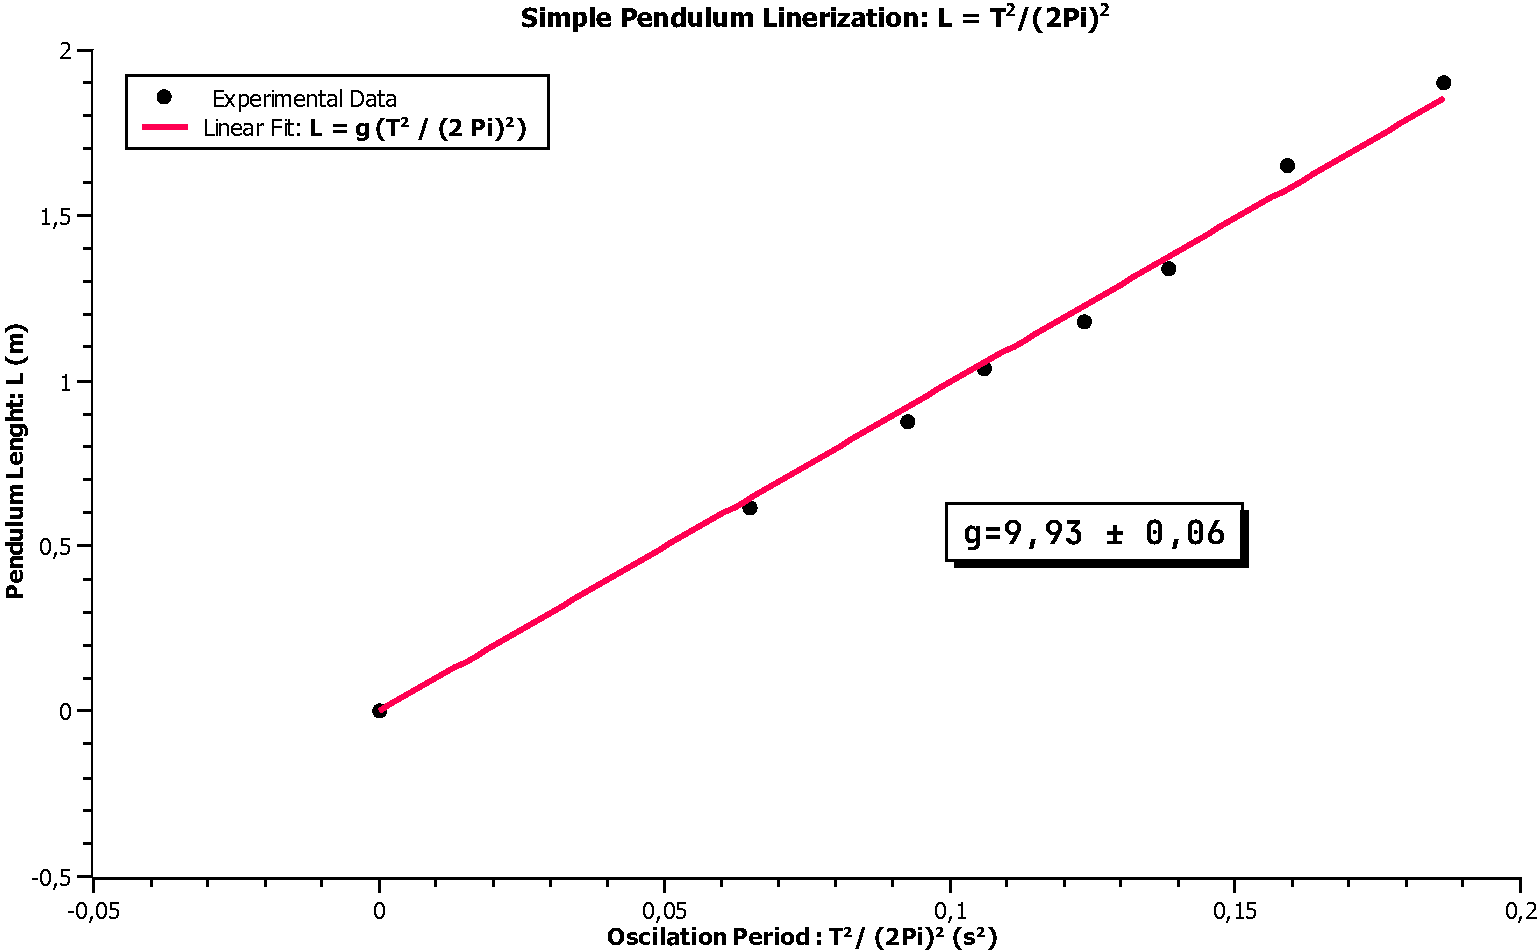
\includegraphics[width=0.8\textwidth]{media/graphs/pendulum_l_1.pdf}
\caption{Ajuste Linear sem constante de ajuste. Fonte: Autor}
\label{fig:ajuste_linear_sem_constante}
\end{figure}
\subsubsection{Log do SciDAVis}
\begin{verbatim}
[sábado, 25 de abril de 2026 11:23:17 Hora oficial do Brasil	Plot: ''Graph1'']
Non-linear fit of dataset: Table1_l, using function: a*x
Y standard errors: Unknown
Scaled Levenberg-Marquardt algorithm with tolerance = 0,0001
From x = 0 to x = 0,186577792296999
a  = 9,93102065416461 +/- 0,0636915352661189
--------------------------------------------------------------------------------------
Chi^2 = 0,0139627645225836
R^2 = 0,998808604394903
---------------------------------------------------------------------------------------
Iterations = 1
Status = success
---------------------------------------------------------------------------------------
\end{verbatim}

Valor encontrado de g a partir do ajuste linear sem constante de ajuste: $g = 9,93 \pm 0,06 \, m/s^2$



\section{Discussão}

Consideramos então, o valor para $g$ encontrado do ajuste sem o termo constante: $g_{exp} = 9,93 \, m/s^2$.

\subsection{Concordância com o Valor de Referência}
Para validar a acurácia experimental, utilizou-se o valor de referência do Observatório Nacional para Belo Horizonte \citep{on_gravimetria_bh_1981}:
\begin{equation}
    g_{bh} = 9{,}7838163 \pm 4\times10^{-7}\,\text{m/s}^2
\end{equation}

O Erro Relativo Percentual ($E_{rel}$) obtido foi de:
\begin{align*}
    E_{rel} &= \frac{|g_{exp} - g_{bh}|}{g_{bh}} \times 100\% \\
\end{align*}
\begin{align*}
\approx \frac{|9,93 - 9,78|}{9,78} \times 100\% \approx 1,53\%
\end{align*}
\section{Conclusão}

O experimento permitiu a determinação da aceleração da gravidade, resultando em $g = 9{,}93 \pm 0{,}06$ m/s$^2$.

A análise dos resultados obtidos a partir dos dois ajustes lineares com e sem constante inicial de ajuste revelou que ambos os modelos forneceram valores para a aceleração da gravidade $g$ que estão próximos do valor esperado de $9,81 \, m/s^2$.

No entanto, o modelo com constante de ajuste apresentou um valor ligeiramente mais alto para $g$, enquanto o modelo sem constante de ajuste apresentou um valor ligeiramente mais baixo. 

A presença da constante de ajuste no modelo pode indicar a existência de um erro sistemático ou uma influência de fatores não considerados no modelo teórico, como a resistência do ar ou a rigidez do fio. 

Por outro lado, o modelo sem constante de ajuste assume que o sistema está idealmente isolado e que todas as condições de contorno são atendidas, o que pode não ser o caso na prática. 

\bibliographystyle{plainnat}
\bibliography{refs}

\end{document}